
%%% Local Variables:
%%% mode: latex
%%% TeX-master: t
%%% End:

\chapter{实例应用}

\section{案例选取}

为了验证本文联合定权方案和误差评定方法的实用性,将其应用到芦山地震中实际反演其震源机制和误差信息。芦山地震发生于2013年4月20日,震级超过$M_w$6级,震源中心在四川省雅安市芦山县附近,是继2008年汶川特大地震以来龙门山断裂带发生的又一强震。地震发生后造成几百人死亡,上万人受伤,受灾人口超过200余万\citep{cuipeng2013},引起了社会各界关注。在直接造成特大地震灾害的同时,芦山地震还诱发了大量的次生地质灾害,其中主要包括落石、崩塌、堰塞湖、泥石流、滚石和滑坡等\citep{chenxiaoqing2013}。这些次生灾害造成的人员伤亡和经济损失也十分巨大,不低于地震的直接影响。

从科学研究的角度看,选取该地震进行方法应用,反演其震源机制有以下两方面优势:首先,芦山地震$M_w$震级在6-7级之间,既可以保证足够的远场地震波能量,同时又可避免过大震级的震源复杂性对波场影响;其次该地震发生后,引起了大量学者的关注,并对其震源机制做了许多研究,有非常多结果可用于与本文方法反演的震源机制进行参考对比,检验结果的可靠性。

\section{反演方案}
反演基于CPS程序的Fit互相关拟合目标函数,利用格点搜索算法进行全空间搜索寻找最优解。为了排除参考震源深度的误差影响,在反演过程中将震源深度也设为可变量,同时加入反演范围。在格点搜索反演中,将震源深度的搜索步长设为1km。而震源机制的搜索则细分为两步,第一步进行全空间快速搜索,将走向、倾角、滑动角的搜索步长均定为10$\degree$,保证求解收敛过程不会陷入局部最优的同时还保证了较高的搜索速度,第二步则进行区域内精搜索,将走向、倾角、滑动角的搜索步长均定为1$\degree$,通过局部范围的少量搜索计算,将最优震源机制的精度提升至1$\degree$。

应用本文误差估计方法评价震源机制误差时,直接将下载的去除仪器响应后的台站数据视为DATA0,然后按照估计方法的流程图进行操作。由于真实地震的震源机制是未知的,不可能像理论实验中比较真值与误差范围的关系一样检验误差是否准确。在此,我们将本地震的误差结果与理论实验的估计误差进行比较、相互印证。之所以可以相互印证是因为刻意设置使得两地震的震源机制相似,虽然使用的观测数据不同,其误差绝对大小也会不同,但是同类型地震各参数间的相关性,以及不同参数的稳定性大小应该是相近的。

为了检验本文提出的WT联合权重在实际应用中的优化效果,设置了三组对照组,分别尝试用WT联合加权、单独W1信噪比加权和单独振幅调节加权W2三种定权方案,对芦山地震的震源机制独立进行反演,并将结果比较分析。对三种加权方案对照组的反演结果评比时综合考虑其结果的稳定性和可靠性。稳定性主要比较反演结果的拟合度高低和震源机制的误差大小。而评价可靠性时,由于无法得知芦山地震震源机制的真值,转而间接考虑可靠性的反面——多解性。如果反演中最优解与其它解差异明显,则表示该解较显著,且有唯一性,较可靠。相反,如果反演过程中搜索到多个极值或性质相近的点,说明具有多解的可能性较大,解不可靠。

\section{数据处理}

在本案例反演过程中,考虑到远震SV波受到其后续波SPL(shear couple wave)的影响,而SPL对地壳上地幔结构敏感,不利于拟合反演,故放弃了SV波,选用远场台站波形中体波P震相和SH震相数据进行震源机制反演。

我们仅使用了远场体波数据,一方面是因为近场波形反演对震源区局部的浅层结构误差敏感,根据\citet{zhenyong2013}和\citet{gaoyuan2013} 的相关研究,发现芦山地震恰巧位于地壳厚度和波速结构横向变化剧烈之处。\citet{xiezujun2013}的研究更直接表明不同一维模型对芦山地震近震反演的震源参数影响高达到10°,而远场波形则对地壳及上地幔的横向非均匀性和震源破裂细节的复杂性不敏感,因而远场数据相对于近场数据更合适于该地震的震源机制反演中。 
另一方面,在前文中提到体波相位的系统性误差理论上可通过平移因子K来抵消,但面波具有频散效应,使得K因子无法很好地补偿结构误差对其相位的影响,且面波易受浅层结构横向非均匀性影响,基于以上考虑,反演时舍弃了面波数据。

在远震情况下,随着震中距增加,地震波的穿透深度越来越深。当震中距接近98$\degree$时,地震波传播路径到达核幔边界,这时将产生绕射波$P_d$,其影响范围如\reffig{fig4_01}所示非常广\citep{Stein2003},但基本在震中距大于98$\degree$的区域。此外,由于核幔边界处的折射作用,在震中距为98$\degree$-145$\degree$的范围内,没有直接穿透的地震波能量到达,该范围内主要受绕射波影响比较大。绕射波在核幔边界的临界条件下产生,对地下结构非常敏感,不适用于震源机制反演。另一方面,为了能将较大地震的破裂面当作点源处理,震中距也不宜太近。
\begin{figure}
\centering
  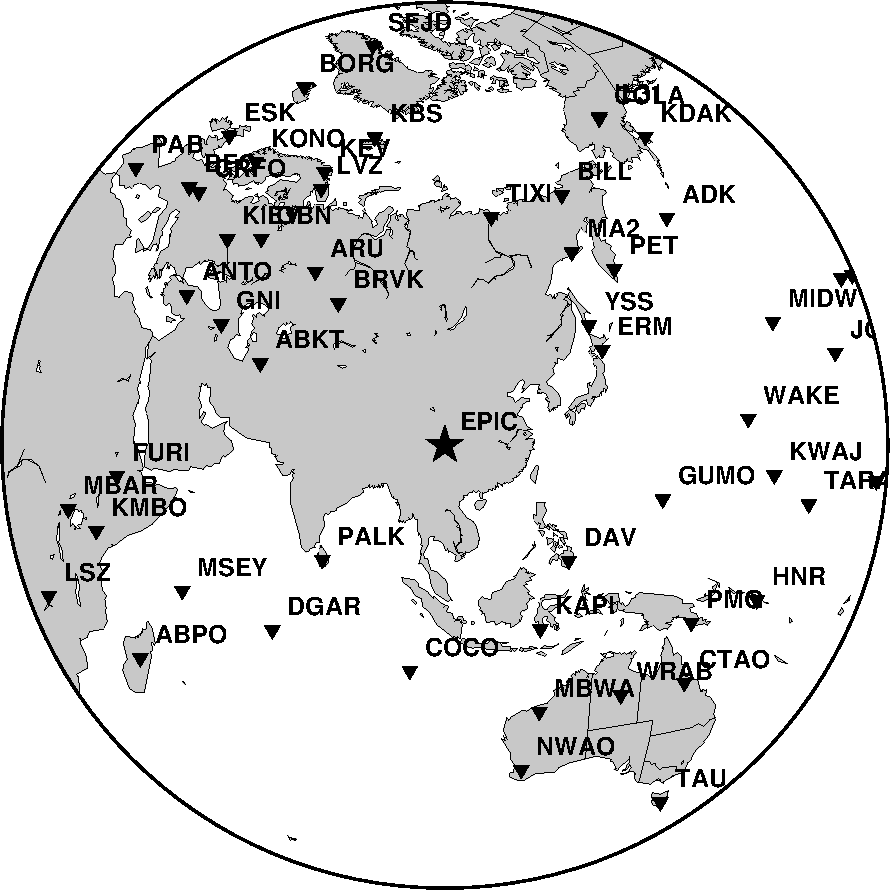
\includegraphics[scale=1.2]{fig4_01.pdf}
  \caption{随着震中距增大,远震情况下绕射波的产生\citep{Stein2003}}
  \label{fig4_01}
\end{figure}


据上分析,本文选取了IRIS提供的54个震中距在30°-90°之间且方位分布较均匀的地震台站(如\reffig{fig4_02}所示),利用这些台站记录的宽频带P波及SH波数据,以ak135模型\citep{Kennett1995}作为地球参考模型通过波形拟合反演震源机制。反演过程中经过多次数据挑选进行除错以提高数据信噪比,最终选取了信噪比较高的102道P震相波形数据和38道SH波波形数据。首先对下载的台站数据进行诸如去除仪器响应、方位旋转等预处理。然后对P波截取了相对P波理论到时(-10s,30s)的时窗,并进行(0.01Hz,0.1Hz)频率范围的带通滤波(该滤波范围基于频谱分析以及多次滤波试验选定)。对38道挑选的SH波数据进行数据处理时,带通滤波频率范围为(0.005Hz,0.06Hz),时窗则选为相对SH波理论到时(-30s,100s)的时间段。
\begin{figure}
\centering
  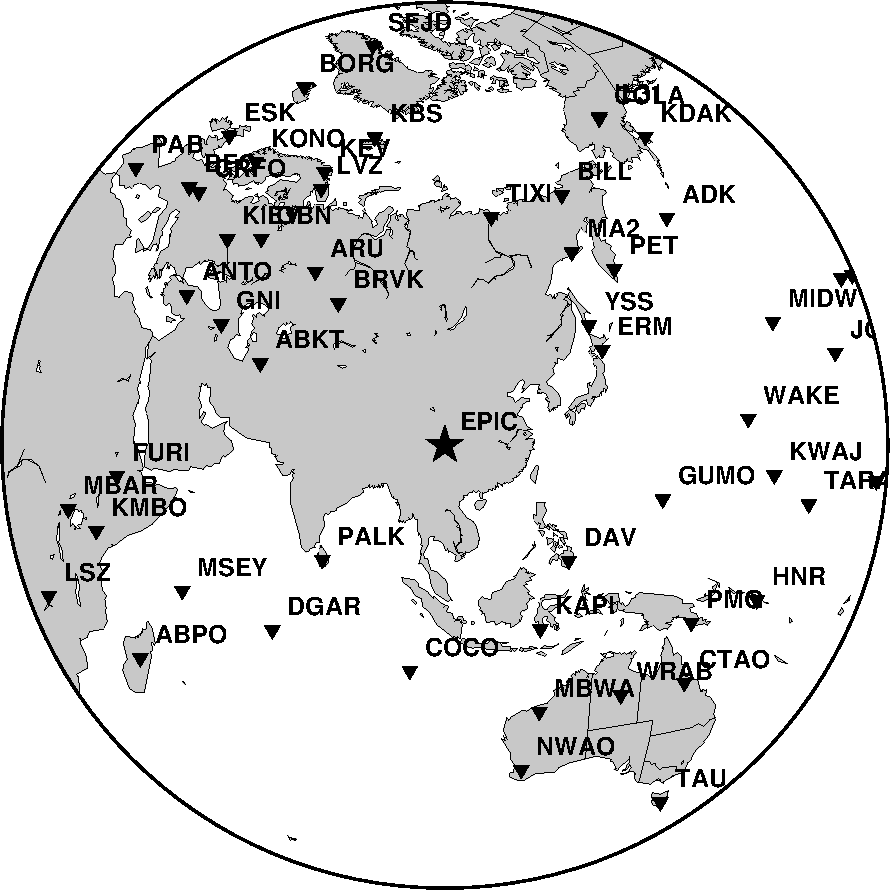
\includegraphics[scale=0.6]{fig4_02.pdf}
  \caption{波形反演所用数据的台站分布,其中五角星表示震中,倒三角表示台站}
  \label{fig4_02}
\end{figure}

\section{反演结果}
三组不同加权对照组反演的震源机制及深度等结果如\reftab{tab4_01}所示,总的来说三次反演结果均较一致,说明该数据分布较理想,结果较稳定,加权起到对反演结果的一种微调作用。
\begin{table}[ht]
\centering
\caption{三种加权方案反演芦山地震的结果}
\label{tab4_01}
    \begin{tabular}{c c c c c c c}
    \hline
    加权方案 & 深度/km  & 走向/$\degree$ & 倾角/$\degree$ & 滑动角/$\degree$ & 震级($M_w$) & 拟合度(Fit) \\
    \hline
    W1		& 16  & 202 & 47 & 96 & 6.49 & 0.7827 \\
    W2		& 18  & 213 & 41 & 95 & 6.41 & 0.5822 \\
    WT		& 17  & 211 & 41 & 94 & 6.41 & 0.6052 \\
    \hline
    \end{tabular}
\end{table}

简单来看,三组对照组中,W1加权组拟合度最高,WT联合加权组次之,而W2加权组拟合度最低。同样的,WT加权组的震源深度结果17km居于另两组震源深度之间,W1加权组和W2加权组的震源深度分别为16km和18km,均只与之相差1km(深度搜索精度为1km)。三组对照组反演的震源机制的三个参数中,走向的差异最大,倾角次之,而滑动角最相近,而从参照组整体来看,W2加权参照组与WT加权参照组的震源机制非常接近,而与W1加权反演组有较明显区别。

\section{分析讨论}
\subsection{结果分析}
首先分析三次反演的拟合度大小以体现W1的作用,从反演理论可知适当增加高质量数据的权重可以减小反演结果的误差,使结果更稳定,并使理论数据与观测值吻合得更好,提升最终的拟合度Fit。从\reffig{fig4_03}所示三组对照组拟合度随深度变化的曲线图,可以发现WT联合加权反演与W2单独加权反演的拟合度曲线非常接近,不过后者的拟合度始终略高于前者。这是因为WT加权反演时对数据信噪比进行了考虑,使得信噪比较低的波形数据在反演中的权重有适当下降,减弱了低信噪比数据中比重较大的随机噪声对反演结果的干扰,同时也使得预测数据与观测数据间的拟合度有所提升。同理,W1单独加权参照组的反演拟合度应是三个参照组中最高的,在\reffig{fig4_03}也能看到W1加权组的拟合度曲线明显高于其它两组。这也是因为W1加权反演组是基于数据随机噪声强度调节权重,为单纯追求反演的拟合度最高,压制了信噪比较低的数据在反演中的作用,而提高了高信噪比数据的贡献,使结果侧重于尽可能满足与高信噪比数据的吻合,最终拟合度也随之提升。此外,对于低振幅的震相,信噪比相对较低,进行W2振幅比调节放大低振幅震相的作用时,也进一步放大了其中的噪声影响,因此数据的整体信噪比会有所下降。因此包含振幅调节加权的两个对照组的拟合度会比W1加权组有较明显的降低,而WT联合加权组的拟合度会比W2加权反演组有所提高。三组反演对照组的拟合度相对大小情况,恰好符合三种加权方案的理论预期效果。
\begin{figure}
\centering
  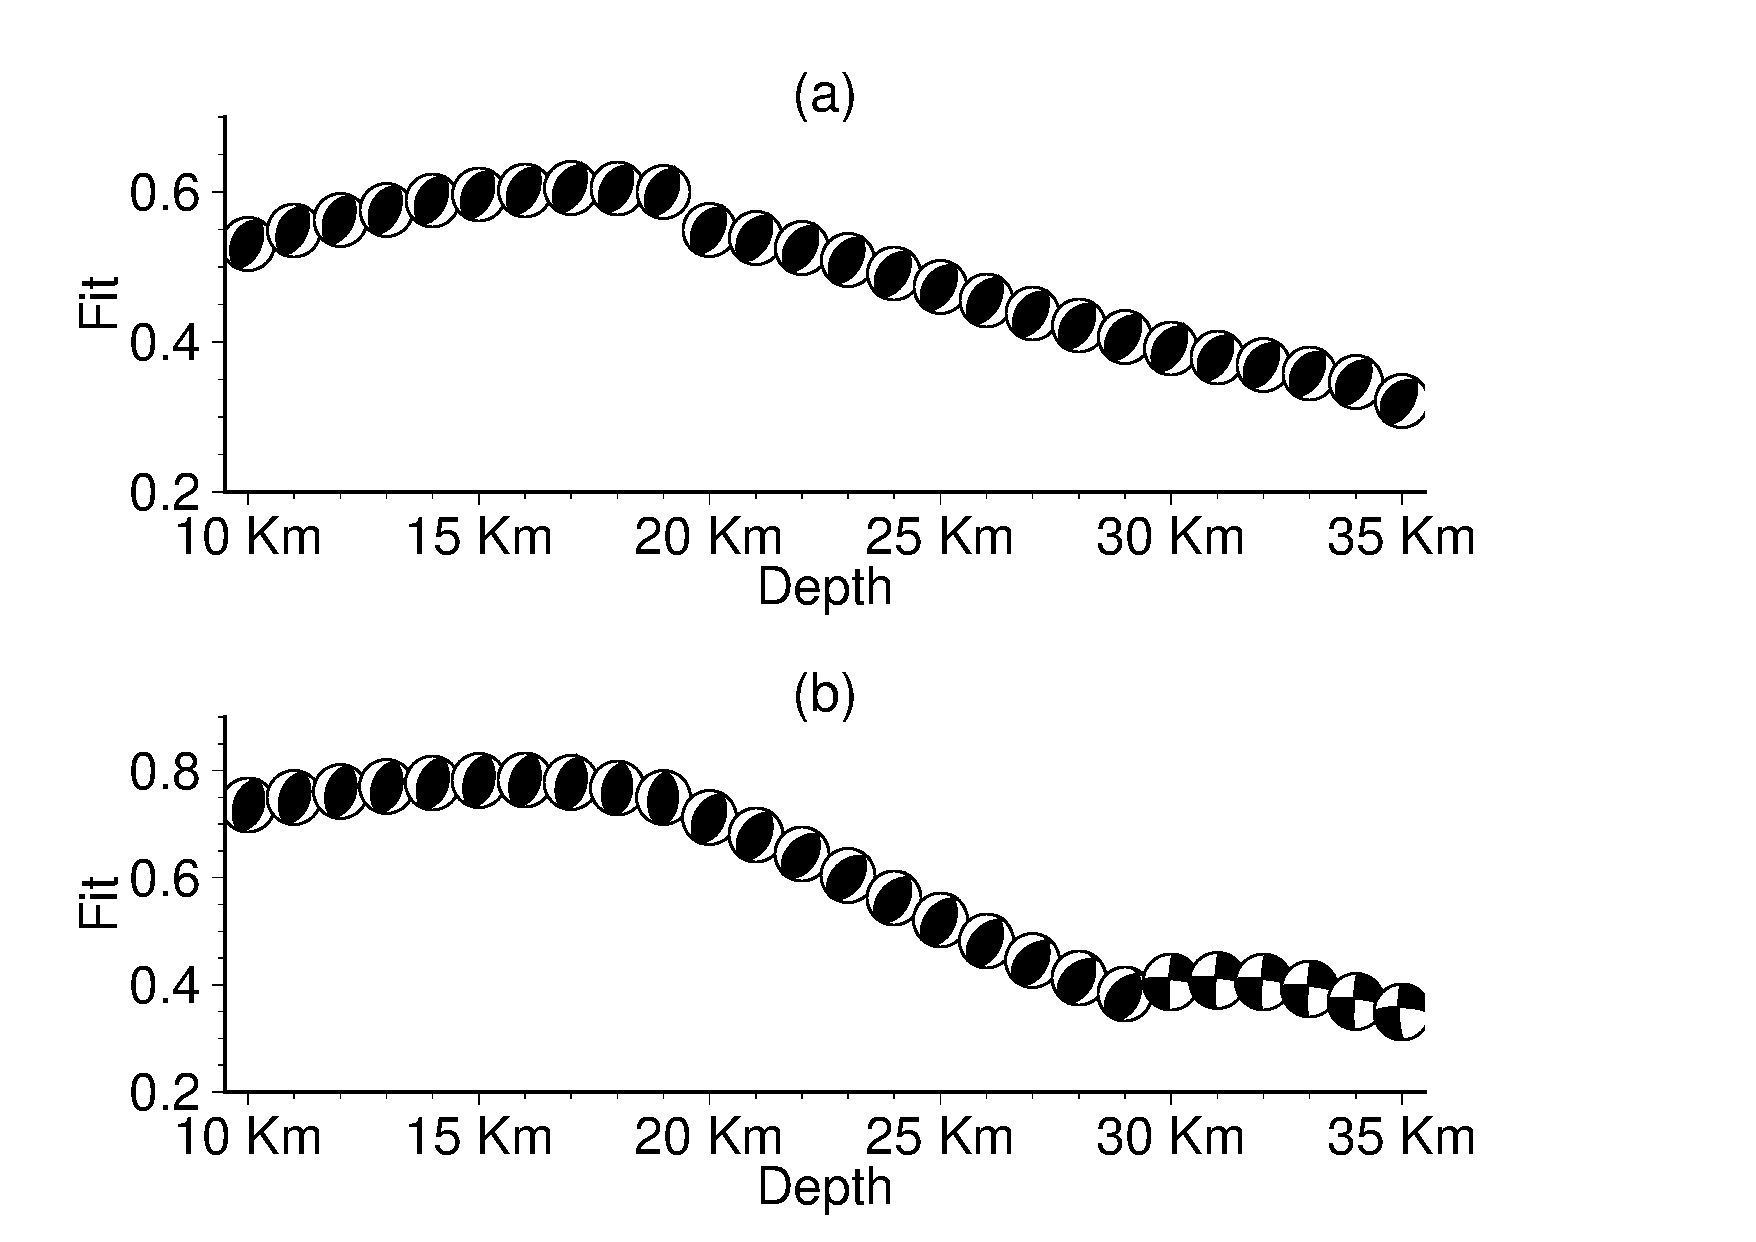
\includegraphics[scale=0.4,angle=0]{fig4_03.pdf}
  \caption{三种反演方案拟合度随震源深度的变化曲线}
  \label{fig4_03}
\end{figure}

前文理论分析中说明了拟合度高低代表了反演结果的稳定性优劣,W1信噪比加权调整了具有信噪比差异的数据在反演中的相对权重,提高了拟合度,抑制了噪声的干扰并增强了结果稳定性。将本文的误差评价方法分别应用于三组参照组,以获得各组震源机制的误差信息,进一步深入对比。为了避免过多的计算量,误差分析过程中重复反演时将震源深度定为第一次用原始观测数据反演的最优深度,因此只需搜索最优走向、倾角和滑动角。三组不同加权对照组的震源机制各参数误差方差如\reftab{tab4_02}所示,可以发现,对应于拟合度最高的W1加权组,其震源机制误差也是三个对照组中最低的,而拟合度最低的W2加权反演组震源机制三个参数的误差都相对其它组大,WT加权组误差大小居中。说明三组对照组反演的震源机制稳定性从优到劣分别为W1加权反演组、WT加权反演组、W2加权反演组,与理论推测完全相符。

\begin{table}[ht]
\centering
\caption{三组加权对照组对应的芦山地震震源机制误差信息}
\label{tab4_02}
    \begin{tabular}{c c c c}
    \hline
    加权方案 & 走向标准差/$\degree$ & 倾角标准差/$\degree$ & 滑动角标准差/$\degree$\\
    \hline
    W1		&  1.03     &    0.00   & 0.61 \\
    W2		&  2.25     &    0.14   & 0.83 \\
    WT		&  1.66     &    0.00	& 0.59 \\
    \hline
    \end{tabular}
\end{table}

但是使拟合度最高的信噪比W1单独加权反演组的震源机制却不见得是三组反演中结果最好的,虽然它具有最好的稳定性,但是对结果的好坏评判还有另一项重要因素——可靠性。以下从震源深度和震源机制的约束效果方面,详细讨论W2振幅调节权重对可靠性的影响。从如\reffig{fig4_03}所示的震源深度格点搜索过程中,可以发现三次反演的全局最值均在18km附近。其中WT反演与W2反演均只有这一个极值,而W1加权反演则在33km附近还出现了另一局部极值,使得解的唯一性不如前两组显著。这说明在同样的反演数据和反演方法情况下,单独进行W1加权的反演对该地震的震源深度约束较差,而包含了振幅调节加权的另两组反演组则对震源深度有较强约束。如前所述,pP及sP震相在远震震相中对深度约束作用最好,在芦山地震波形进行低频滤波数据处理情况下,pP及sP深度震相与P震相交叠在一起,pP和sP的信息包含在P波时窗中,故“P波”数据对震源深度约束较好。而对于接近剪切位错源的大多数天然地震,S波振幅通常比P波振幅大很多,未经W2振幅调节会导致P波的信息在反演中得不到充分体现,反演结果侧重于关注S波的拟合。因而导致三组不同加权反演对照组中,单独W1信噪比加权反演组对震源深度的约束效果相较于另两次反演最差。

另一方面,从\reffig{fig4_04}可以看到,W1单独加权组与WT联合加权对照组在第一次对原始观测数据DATA0进行包含震源深度搜索的震源机制反演过程中,不同深度对应的最佳震源机制情况。很明显WT联合加权组在深度搜索过程中不同深度对应的最佳震源机制一直较为稳定,而W1单独加权反演中不同深度对应的最佳震源机制差异较大,甚至在震源深度全局最值附近,各深度对应最优走向的变化也较为显著。这表明WT联合加权反演的震源机制,其解的唯一性比W1单独加权反演要好,结果更可靠。这是因为W2权重更好地平衡了不同振幅波形在反演中的影响,使得各种震相信息在反演中得到合理的充分利用,相当于间接改善反演数据的数据结构,从而能更有力、更全面地约束待反演的所有参数。
\begin{figure}
\centering
  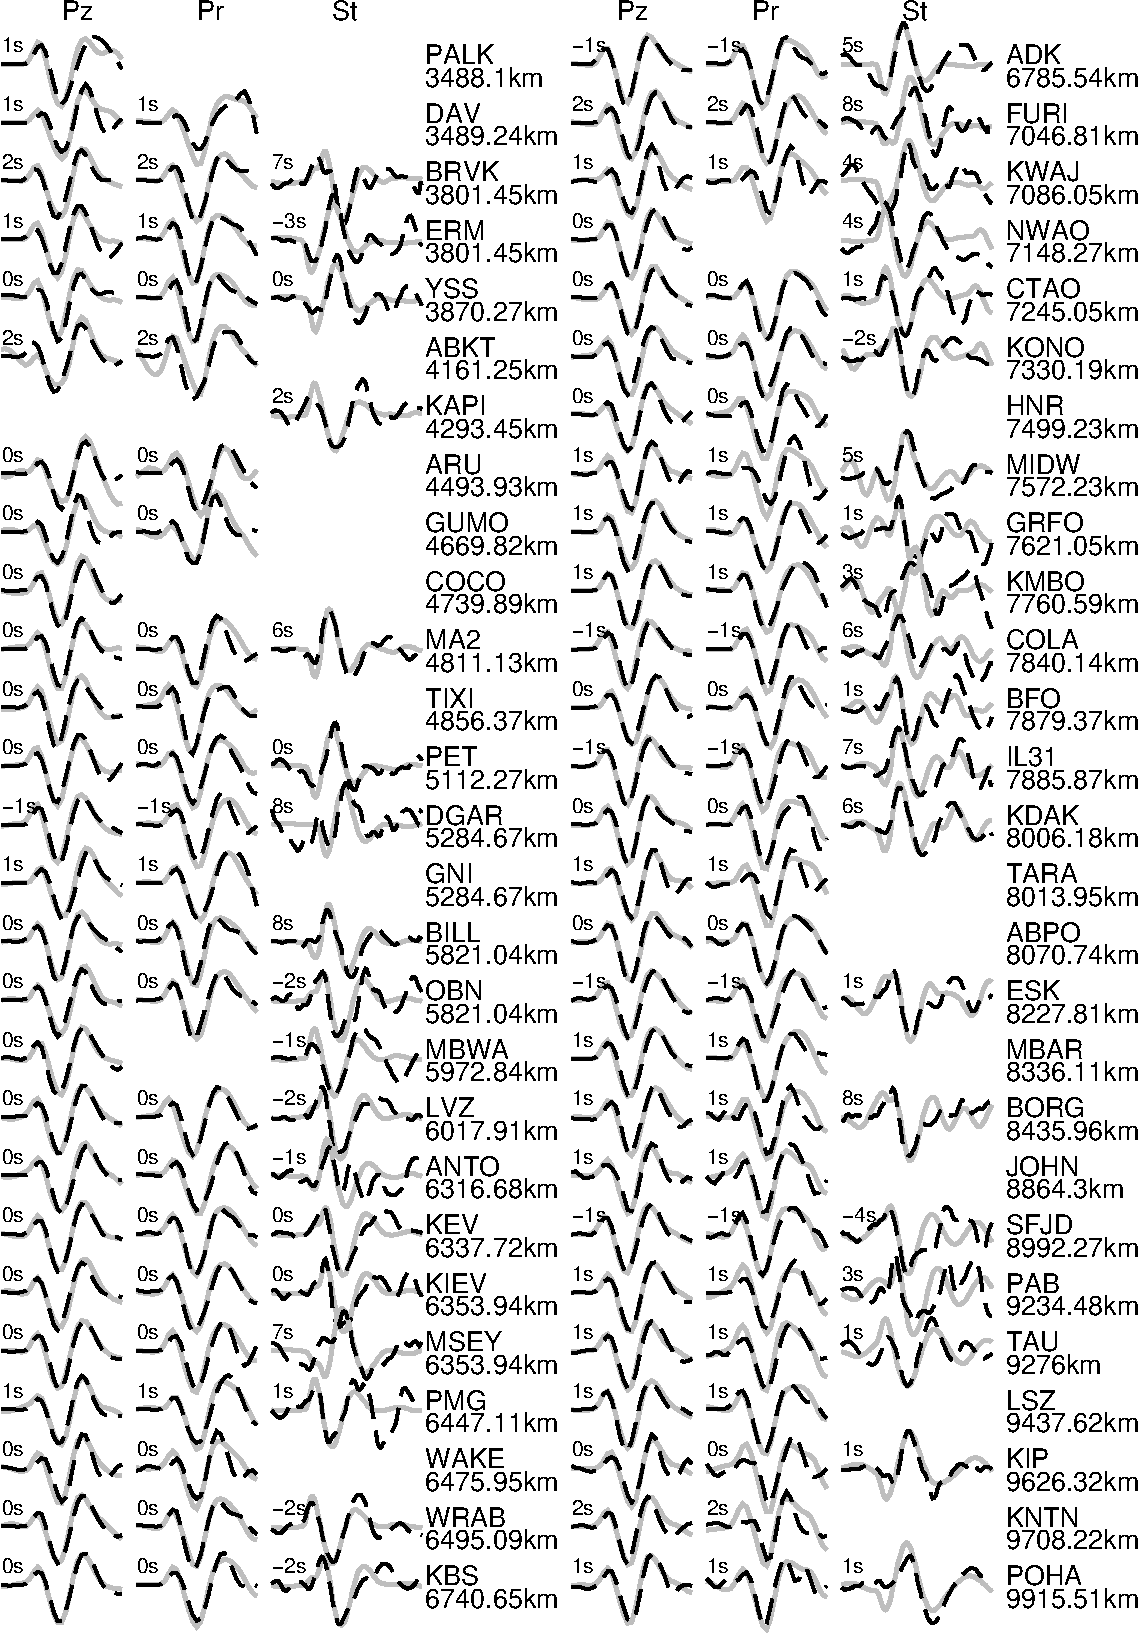
\includegraphics[scale=0.4]{fig4_04.pdf}
  \caption{ (a)(b)分别为wt(WT)加权W1加权反演各震源深度对应最佳解}
  \label{fig4_04}
\end{figure}

综上分析,W1信噪比加权通过压制高噪数据,提高反演数据的整体信噪比,能有效减弱随机噪声对反演结果的影响,增强了结果稳定性;W2振幅调节加权合理分配权重给具有振幅差异的震相波形,使反演充分利用各种震相信息,间接改善了数据结构,更好约束了反演结果,提升了结果的可靠性。

在反演时若仅考虑信噪比加权,虽然能提高结果稳定性,但是可靠性偏低,甚至出现多解情况;相反,单独考虑振幅调节加权则会降低结果稳定性。WT联合加权的效果相对更全面地考虑了结果稳定性和可靠性,在保证结果可靠性的同时,获得了较优良的稳定性,表明WT加权组的反演结果应该是三组反演组中综合效果最优的。将WT联合加权反演组的反演结果视为本文芦山地震反演的最终结果,假设误差不超过其三倍标准差大小,并结合搜索步长为1$\degree$的精度,根据\reftab{tab4_02}得到最终包含误差估计的震源机制为(走向$211\degree\pm5\degree$,倾角$41\degree\pm1\degree$,滑动角$94\degree\pm2\degree$)。

WT联合加权反演的最优震源机制所对应的所有台站理论与观测波形拟合情况如\reffig{fig4_05}所示。可以看到P波及SH波拟合得都不错,相位及其振幅均匹配得非常好。值得注意的是,同一台站的P波Z与R分量的时间平移参数非常一致,这是因为平移因子是由地震定位,发震时刻及地球速度结构等系统性误差引起的,且理论上其误差影响对于同一台站的同一震相应是相同的。此外,对于不同震中距台站的波形,拟合情况均相当,表明反演综合考虑了所有波形的信息。
\begin{figure}
\centering
  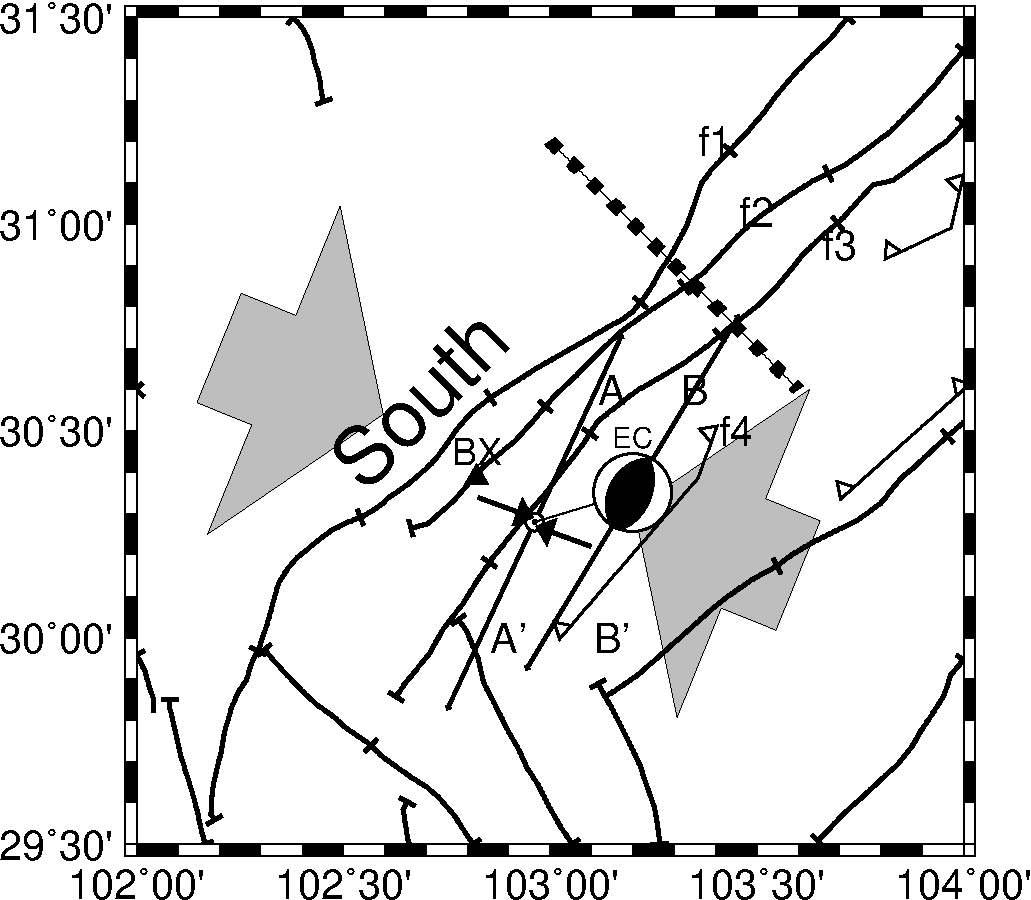
\includegraphics[scale=0.78]{fig4_05.pdf}
  \caption{ wt加权反演波形对比图,虚线为观测波形,实线为理论波形,波形右侧分别为台站名、震中距(km)。各道波形的左上方为到时差,正值表示理论到时相比实测波提前,负值相反}
  \label{fig4_05}
\end{figure}

通过本文的误差评价方法,可以得到最终震源机制的三参数间相关系数,将其列于\reftab{tab4_03}中。从之前的理论实验中,已经发现对于相同的震源机制,即使反演数据源有差异,其各参数间的相关系数仍较为相近,具有可比性。本文理论实验中所用的震源机制与反演所得的芦山地震震源机制较为相近,因此理论上其震源机制参数的相关系数也应相似。对比\reftab{tab4_03}与之前理论实验中不同噪声数据反演组对应的震源机制相关系数,可以发现芦山地震震源机制的走向和滑动角也与之前理论实验一样,体现了较强的正相关性,而倾角和另两参数的相关性相对较为不明显,基本情况近似吻合。
\begin{table}[ht]
\centering
\caption{芦山地震震源机制各参数间相关性}
\label{tab4_03}
    \begin{tabular}{c c c c}
    \hline
    相关系数 & 走向/$\degree$ & 倾角/$\degree$ & 滑动角/$\degree$ \\
    \hline
	走向/$\degree$ 		&1 			&0			&0.91\\
	倾角/$\degree$		&0			&1			&0\\
	滑动角/$\degree$	&0.91		&0			&1\\
    \hline
    \end{tabular}
\end{table}

另一方面,对于三参数中各自误差的相对大小,也可以发现,理论实验和芦山案例中震源机制倾角的误差均是最小的,走向的误差均较大。说明走向、倾角和滑动角误差的相对大小是和震源机制类型密切相关的。

芦山地震案例反演中,震源机制相关系数,和各参数误差相对大小的情况,与理论实验均有较高相似性,从侧面反映了对芦山地震估计的震源机制误差信息是较准确的。

\subsection{其它震源研究}

芦山地震后,各研究者分别对该地震震源机制进行了详细研究。\citet{zengxiangfang2013}利用\citet{Hardebeck2002}改进的P波初动极性反演方法及近远震波形反演方法得到了较一致的震源机制解,且借助误差曲线利用阈值类方法分析了倾角和深度的可靠性;\citet{liujie2013}、\citet{lujian2013}利用CAP方法对近震波形反演得到了芦山地震震源机制解,其中吕坚在波形反演基础上利用余震分布进一步约束了发震断层面;\citet{xiezujun2013}利用CAP方法分别对近震、远震及近远震联合反演进行对比以得到最佳震源机制。

相关研究所反演得到的震源机制均列于\reftab{tab4_04}中,可发现不同研究者所得到的结果分布情况,震源深度范围为(12km-22km),震源机制走向范围(200$\degree$-220$\degree$),倾角范围(33$\degree$-50$\degree$),滑动角范围(90$\degree$-110$\degree$),$M_w$震级(6.4-6.7)。本文反演的最终结果(震源深度17km,走向$211\degree\pm5\degree$,倾角$41\degree\pm1\degree$,滑动角$94\degree\pm2\degree$,$M_w$震级6.41)基本在此分布范围内,仅$M_w$震级略小。这一方面可能是由于本文的Fit函数的特性,为了降低系统性误差对震源机制的影响,将振幅误差归并到了震级评估中;另一方面因为各学者所用的数据及参考模型不尽相同,并且除了速度结构、地震定位以及发震时刻的不精确,理论波形的计算方法也可能导致系统性误差,相关研究表明不同程序算得的理论波形相位一致性较好,但振幅则会有一定可见差异\citep{Herrmann1985}。

\begin{table}[ht]
\newcommand{\tabincell}[2]{\begin{tabular}{@{}#1@{}}#2\end{tabular}}
\centering
\caption{不同研究者得到的芦山地震震源机制,参考自\citet{lujian2013}}
\label{tab4_04}
    \begin{tabular}{c c c c c c c c c c c }
    \hline
    研究者 & \tabincell{c}{美国\\地调\\局} & \tabincell{c}{Global\\CMT} & \tabincell{c}{刘超\\等} &\tabincell{c}{韩立\\波等} &\tabincell{c}{中国地\\震局预\\测所} & \tabincell{c}{刘杰\\等} & \tabincell{c}{曾祥\\方等} & \tabincell{c}{谢祖\\军等} & \tabincell{c}{吕坚\\等} & \tabincell{c}{本文\\结果}\\
    \hline
	深度/km			&12	&22	&15	&12	&15	&19	&12	&16	&14	&17 \\
	走向/$\degree$	&198&210&220&220&210&214&212&210&209&211\\ 
	倾角/$\degree$	&33	&38	&35	&50	&47	&39	&47	&44	&46	&41	\\
	滑动角/$\degree$&71	&96	&95	&107&90	&100&93	&91	&94	&94	\\
	$M_w$			&6.6&6.6&6.7&6.6&6.5&6.4&6.7&6.7&6.6&6.4\\
    \hline
    \end{tabular}
\end{table}

各研究者所得的震源深度跨度较大,\citet{gaoyuan2013}对地震重定位得到主震震源深度17.8km,\citet{fanglihua2013}用三维速度模型进行双差重定位给出的震源深度为17.2km和17.6km,其中房立华使用了接近震中附近的三维速度模型,并用流动观测台站对早期发生的地震进行校正,结果是较为可信的。各研究者的震源矩中心深度相对重地位的破裂点深度差异绝对值不超过5km,考虑到超过$M_w$6级的地震强度,破裂面延展可能较大,故差异相对可以接受,而本文反演的震源深度17km也是较为合理的。

\subsection{相关地质背景}
芦山地震震源位于龙门山断裂带,在该区域由于同时受到西北部青藏块体向东的挤压作用,以及东南部四川盆地坚硬地壳的阻挡,使得青藏块体东缘下方的地壳物质东流,进而导致较软弱的下地壳物质向上逆冲挤出,最终形成逆冲型的东南走向的龙门山断裂带\citep{Zhang2013}。该断裂带主要由4条大断裂构成\citep{dengqidong1994,lizhiwu2008},其整体走向为SW向。可是从整体来看,该断裂带南北段走向具有明显的差异性\citep{Jia2006,Arne1997,guozhengwu1996,dengkangling2007},芦山地震震源区所处的南段走向相较于北段而言,有更南偏倾向。龙门山断裂带南段因受喜马拉雅期印-亚碰撞事件的重大影响,显示与松潘-甘孜褶皱带有密切关系,推断其为晚白垩世古近纪沉降中心,南段的断裂活动性延续时间较晚,直到喜马拉雅期基本定型,但现今仍在发育\citep{lizhiwu2008}。

龙门山断裂带区域的构造及地下结构一直是大家研究的热点,相关研究成果\citep{Zhang2013,Wang2010,zhangzhongjie2009,Zhang2011,leijianshe2009}表明,龙门山地区的地壳速度结构处于横向变化剧烈处,存在明显的不均匀性,而芦山地震的震源恰巧在P 波速度变化较大的区域。芦山地震震中与龙门山断裂带南段断层分布(断层数据来自\citet{dengqidong2002})如\reffig{fig4_06}所示,由图可知震中位于南段前山断裂和山前隐伏断裂之间,地质调查结果\citep{xuxiwei2013}显示芦山地震的发震断层为一条现今尚未出露地表、其上断点仍埋藏在地下地壳中的一条盲逆断层,无法直接从地表露头来观测震源断裂处走向情况,但是本文反演得到的震源机制显示的走向211°与震源区域断层整体走向基本吻合,表明反演得到的走向具有合理性。此外,相关研究\citep{tangchangrong1991,liyong2006,Densmore2007,chenguoguang2007}表明龙门山断裂带总体运行表现为为由北西向南东的逆冲 ,并且同时兼具有右旋走滑的特性, 整条断裂带的冲断运动由北西向南东扩展,但由于受到后山、中央、前山三条断裂带的阻碍作用,断裂带的北段和中段的山前断裂并没有明显地显现出逆冲的特征,可是芦山地震所处的南段区域却不同,其山前断裂带明显受到了冲断运动的影响,发生了较为强烈的冲断和摺皱变形,为震源所处的盲逆断层孕震提供了有利条件,与本文反演得到的滑动角所代表的逆冲型断裂发震的运动背景一致。
\begin{figure}
\centering
  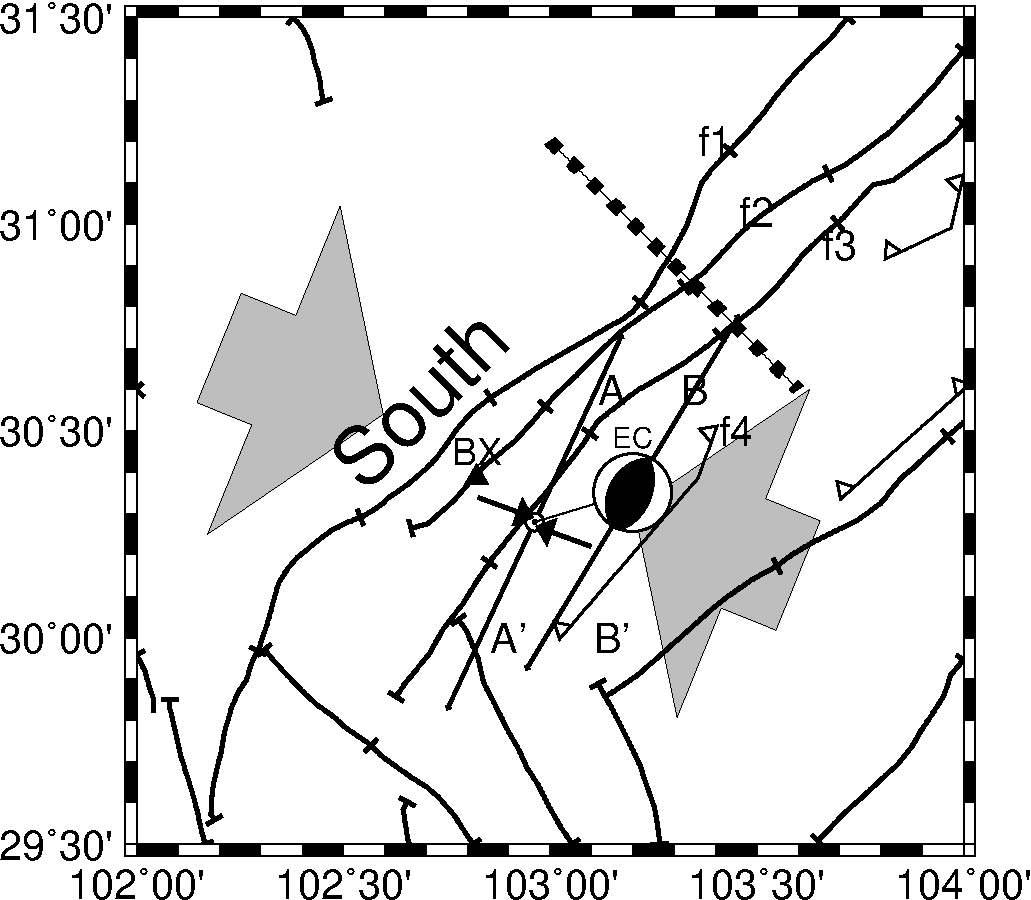
\includegraphics[scale=0.6]{fig4_06.pdf}
  \caption{ 震源区域断层与应力分布, f1,f2,f3,f4为龙门山断裂带的主要四大断裂,灰色大箭头为区域平均应力,黑色小箭头为本文震源机制对应的主压应力}
  \label{fig4_06}
\end{figure}

由于芦山地震发震断裂为盲断裂,难以直接观测发震断裂的空间构造,通过余震分布可以一定程度重现发震断裂的结构信息,\citet{zhangguangwei2013}通过双差定位发现在空间分布上主震西南方向余震分布较广、且较为集中,余震主要向西南方向扩展(\reffig{fig4_06}中AA'剖面),其剖面方向与本文震源机制的走向线BB'近乎平行,说明余震基本沿主震断层面破裂分布。

断层构造活动通常与该区域的应力分布有着密切关系,\citet{mengwen2013}实地钻孔测量研究结果表明龙门山断裂带的水平应力占主导作用,且南段的优势方向为NWW向。根据青藏高原内部存在下地壳通道流的观点\citep{Royden1997,Clark2000,Meng2005,Burchfiel1995,Harris2007},松潘-甘孜地体极有可能俯冲到四川盆地之下\citep{louhai2010},从而使得龙门山断裂带南段与青藏高原东部具有较好的连接性,是青藏高原东缘的活动边界,因此龙门山断裂带南段最大主压应力方向与区域应力场方向一致,为NW-NWW向,孟文等的钻井数据显示距震中较近的宝兴钻井点主应力方向为N80°W至N74°W,另一钻井结果表明宝兴主应力方向为N60°W\citep{qinxianghui2013},上述区域应力方向以及实际钻井没得的主应力方向均与本文反演所得的震源机制主应力方向一致。

研究表明, 快剪切波偏振的优势方向一般与原地主压应力方向一致\citep{Gao2011,Gao2012},\citet{gaoyuan2013}用剪切波分裂的方法计算发现位于芦山地震震中东北方向的龙门山断裂带中南段的台站快剪切波偏振的优势方向近似为NW 向,与断裂带走向近似垂直;而在芦山地震震中西南方向的龙门山断裂带南段靠近鲜水河断裂处,快剪切波偏振方向表现得比较离散,但平均方向为近EW方向,所以地理位置位于其中间的震中区的偏振优势方向极有可能在NW与EW之间。此外\citet{zhaobo2013}利用力轴张量法计算得到的芦山地震余震分布区的平均压应力方向约为112°,如\reffig{fig4_06}中灰色大箭头所示。本文震源机制(走向211°,倾角41°,滑动角94°)对应的P轴近水平,与各向异性分析及力轴张量计算法得到的应力结果有很好的一致性。上述钻井实测资料,应力计算资料结果相互吻合,均与本文震源机制表现出一致性,表明芦山地震主要为区域NWW向水平应力长年积累的一次应力释放。

\section{结论}
芦山地震实例反演中,震源机制误差大小与不同加权稳定性的预测一致,且该案例中三参数误差的相对大小和它们之间的相关性,与相近地震类型的理论事件情况相似,均表明对芦山地震震源机制的误差估计较可靠,证明了本文误差估计方法在真实地震案例中的实用性。

根据不同加权的三组反演对照组的对比结果,W1信噪比加权抑制了噪声干扰,明显提高了拟合度,并且减小了结果误差,增强了稳定性。W2振幅调节加权合理为振幅不同的震相分配权重,间接优化了数据结构,防止了33km震源深度附近极值点的出现,减弱了结果的多解性,增强了结果的可靠性。WT联合反演吸收了W1和W2的优点,全面考虑了数据信噪比和数据结构,综合提升了结果的稳定性和可靠性。

本文反演芦山地震的最终结果——震源深度17km,震源机制(走向$211\degree\pm5\degree$,倾角$41\degree\pm1\degree$,滑动角$94\degree\pm2\degree$),与其它研究者的结果有良好一致性,且与震源区域的地质构造背景和应力情况相符合,表明本文反演结果较为可信。根据应力分布、地震定位及构造情况,推断本次地震震源为由区域水平向应力长期积累下的势能释放,导致的高倾角近纯逆冲型滑动断裂。
